\documentclass[12pt,a4paper]{article}
\usepackage[utf8]{inputenc}
\usepackage{amsmath}
\usepackage[brazilian]{babel} % Brazil or not Brazil??
\usepackage{amsfonts}
\usepackage{amssymb}
\usepackage{graphicx}
\usepackage[margin=0.8in]{geometry}


\begin{document}
\title{\vspace{70mm}\Huge Experimento 04 - Máquina de atwood}
\author{ Giovani Garuffi\qquad\hfill
		\textit {RA: 155559}\protect\\
		João Baraldi\hfill
		\textit{RA: 158044}\protect\\
		Lauro Cruz\hfill
		\textit{RA: 156175}\protect\\
		Lucas Schanner\hfill
		\textit{RA: 156412}\protect\\
		Pedro Stringhini\hfill
		\textit {RA: 156983}								
		}
\maketitle
\newpage
\section{Resumo}
Inicialmente, prendeu-se um fio (inextensível) com duas massas nas extremidades em uma polia em torno de um eixo fixo (Máquina de Atwood). Após variar a diferença entre as massas das extremidades dos pesos dos fios (com discos de metal de massas variadas) e obter os períodos de queda de da massa de maior peso com um cronômetro, foi utilizada a fórmula $Delta m = (\frac{2h}{gR^2})(I + MR^2))(\frac{1}{t^2})+(\frac{tau_a}{gR})$ para determinar o momento de inércia da polia e o torque do atrito.
Após a transformação linear da equação em X, traçou-se um gráfico de Y por Z. A partir desses dados e das dimensões do cilindro (calculadas com um paquímetro), foi possível a determinação do momento de inércia aproximado a partir da fórmula X_2.
% Não me lembro das fórmulas e dos eixos do gráfico, sei q sou várzea, mas me ajudem ;) hahahaha

\section{Objetivos}
O experimento realizado teve como objetivo estudar a máquina de Atwood, utilizando para isso a determinação do momento de inércia da polia utilizada e do torque realizado pelo atrito entre tal polia e o fio que a toca.$T = \sqrt{\frac{8\pi I_0 L}{G r^4}}$


\section{Procedimento Experimental e Coleta de Dados}

\subsection{Materiais utilizados}

\begin{itemize}
	\item Polia de latão com eixo;
	\item barbante;
	\item dois pesos de suspensão;
	\item vários discos metálicos que se acoplam aos pesos;
	\item fita métrica para medição de comprimentos;
	\item paquímetro;
	\item balança de precisão;
	\item cronômetro;
\end{itemize}

\subsection{Procedimento}





\subsection{Dados Obtidos}


\section{Análise dos Resultados e Discussões}
\subsection{Regressão linear}
Pela equação 

$$\Delta m = \frac{2h}{gR^2} \cdot (I + MR^2)\dfrac{1}{t^2}  + \frac{\tau _a} {gR}$$
Onde $\Delta m = m_1 - m_2$, $ M = m_1 + m_2 $, $h$ é a altura inicial, $t$ é o tempo em que os corpos se deslocam de $h$, $I$ é o momento de inércia do cilindro de latão, $R$ é o seu raio.\\
Vemos que existe uma relação linear entre $\Delta m$ e $ \dfrac{1}{t^2}$. Para explorar essa relação, foi construída a Tabela \ref{linear}, relacionando $\Delta m$ à $ \dfrac{1}{t^2} $ .

\begin{table}[!htbp]
\centering
\def\arraystretch{1.5}
\caption{A diferença de massa, relacionada à grandeza $1/t^2$.}
\begin{tabular}{|c|c|c|}
\hline 
$\Delta m \; (g)$ & $t \; (s)$ & $1/t^2 \; (s^{-2})$ \\ 
\hline 
$37.0 \pm 0.1$ & $4.24 \pm 0.03 $ & $0.055 \pm 0.001 $  \\
\hline
$29.2 \pm 0.1$ & $4.51 \pm 0.05 $ & $0.049 \pm 0.001$ \\
\hline
$10.2 \pm 0.1$ & $8.34 \pm 0.05 $ & $0.0143 \pm 0.0002$\\
\hline
$10.4 \pm 0.1$ & $8.60 \pm 0.09 $ & $ 0.0135 \pm 0.0003 $\\
\hline
$9.8 \pm 0.1$ & $8.51 \pm 0.01 $ & $ 0.01379 \pm 0.0002 $\\
\hline
$13.6 \pm 0.1$ & $7.26 \pm 0.03 $ & $ 0.0189 \pm 0.0003 $ \\
\hline
\end{tabular} 
\label{linear}
\end{table}
Fazendo a regressão linear de $ \Delta m$ X $ \dfrac{1}{t^2} $, pelo método de mínimos quadrados, obtem-se os seguintes coeficientes: 
	$$ a = 0.00138 \pm 0.00005 $$
	$$ b = 0.0002 \pm 0.0005 $$

A reta resultante da regressão linear, sobreposta aos pontos medidos experimentalmente pode ser vista na Figura \ref{grafico}. Nota-se que o experimento falhou em coletar dados distribuidos uniformemente sobre o eixo $ \Delta m$, e isso pode acarretar erros e incertezas.

\begin{figure}
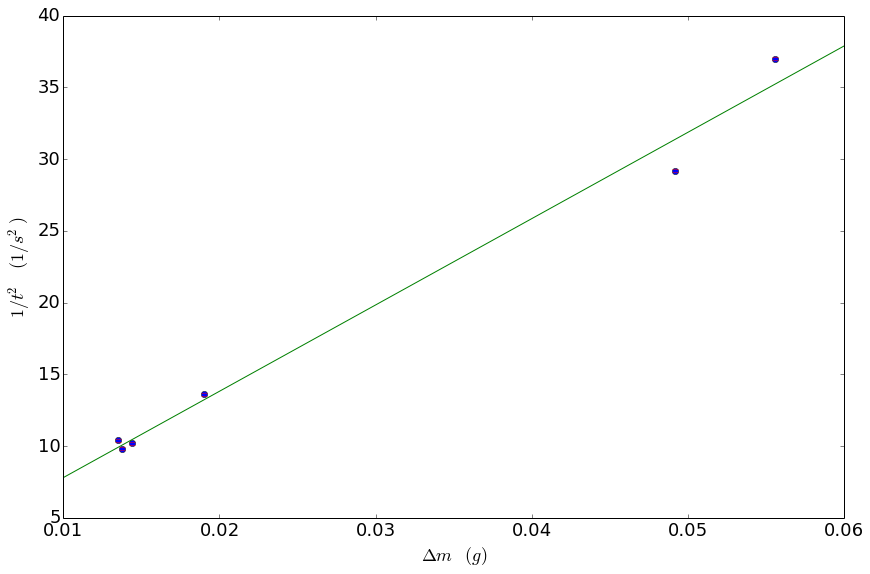
\includegraphics[scale=0.55]{grafico.png}
\caption{Regressão linear de $\Delta m$ por $1/t^2$ sobreposta aos pontos experimentais}
\label{grafico}
\end{figure}

\subsection{Significado do coeficiente angular}

\section{Conclusões}




\end{document}

